\documentclass[10pt,twocolumn,letterpaper]{article}
\usepackage[CJKchecksingle,CJKnumber]{xeCJK}
\setCJKmainfont[BoldFont={SimHei},
ItalicFont={KaiTi}]{SimSun}
\usepackage{cvpr}
\usepackage{times}
\usepackage{epsfig}
\usepackage{graphicx}
\usepackage{amsmath}
\usepackage{amssymb}

% Include other packages here, before hyperref.

% If you comment hyperref and then uncomment it, you should delete
% egpaper.aux before re-running latex.  (Or just hit 'q' on the first latex
% run, let it finish, and you should be clear).
\usepackage[pagebackref=true,breaklinks=true,letterpaper=true,colorlinks,bookmarks=false]{hyperref}

\cvprfinalcopy % *** Uncomment this line for the final submission

\def\cvprPaperID{****} % *** Enter the CVPR Paper ID here
\def\httilde{\mbox{\tt\raisebox{-.5ex}{\symbol{126}}}}

% Pages are numbered in submission mode, and unnumbered in camera-ready
%\ifcvprfinal\pagestyle{empty}\fi
\setcounter{page}{1}
\begin{document}

%%%%%%%%% TITLE
\title{Learning realistic human actions from movies\\}

\author{Ivan Laptev\\
INRIA Rennes,IRISA\\
{\tt\small ivan.laptev@inria.fr}
% For a paper whose authors are all at the same institution,
% omit the following lines up until the closing ``}''.
% Additional authors and addresses can be added with ``\and'',
% just like the second author.
% To save space, use either the email address or home page, not both
\and
Marcin Marszalek~~~~~~Cordelia Schmid\\
INRIA Grenoble,LEAR-LJK\\
{\tt\small marcin.marszalek@inria.fr~~~~~~cordelia.schmid@inria.fr}
\and
Benjamin Rozanfeld\\
Bar-Ilan University\\
{\tt\small grurgrur@gmail.com}
}

\maketitle
%\thispagestyle{empty}

%%%%%%%%% ABSTRACT
\begin{abstract}
   这篇文章的目的是处理多样化以及现实生活的视频场景设定中的人类行为识别问题。
   这项困难但是重要的课题在过去因为诸如缺乏现实标记的视频数据集等问题被忽视。
   我们的第一项工作是处理数据集的限制,研究使用电影剧本来自动标注视频中的人类
   行为。同时我们评估了其它可选的行为恢复方法进行比较并展示了基于文本的分类器的
   优势。采用恢复出来的行为样本进行视觉学习,然后我们继续处理视频中行为分类的问题。
   我们提出了一种新的基于视频的分类方法,这些方法依赖和扩展于一些近来提出的方法,
   包括局部空域-时域特征,空域-时域金字塔以及多通道非线性支持向量机。我们提出的
   方法与其它具有代表性的技术相比在标准KTH行为数据集上将精确度提升到了91.8\%,而且
   我们特别研究并展现了我们的方法对于训练数据集标注错误的非常高的耐受性。最后,我们
   将方法应用到电影中具有挑战性的行为类别上,呈现出可观的结果。
\end{abstract}

%%%%%%%%% BODY TEXT
\section{引言}
在过去的十年中视觉识别领域从分类玩具对象实例发展到识别自然图像中多种类的对象和场景,有了显著的进步。
这受益于现实的图像数据集的创建以及新的鲁棒的图像描述和分类方法。我们从这一进程中受到启发,计划将先前
的经验转换到视频识别和人类行为识别的领域中。

已有的人类行为识别数据集(例如\cite{15},见图8)只提供了处于控制和简化的场景设定下记录的较少的行为类别。
这和现实生活应用要求的处理包含具有个体差异的人类行为的自然视频有很大差异,这些个体差异来源于
表情,姿势,动作和衣着,透视效果和镜头运动,明亮度差异,以及场景遮挡和变化等。这篇文章中我们将处理
当前数据集的限制,采集现实视频中的人类行为样本(如图1所示)。特别地,我们考察人工视频标注的困难并提出
自动标注电影中的人类行为的基于剧本对齐和文本分类的方法(第2节)。

\begin{figure}[t]
\begin{center}
   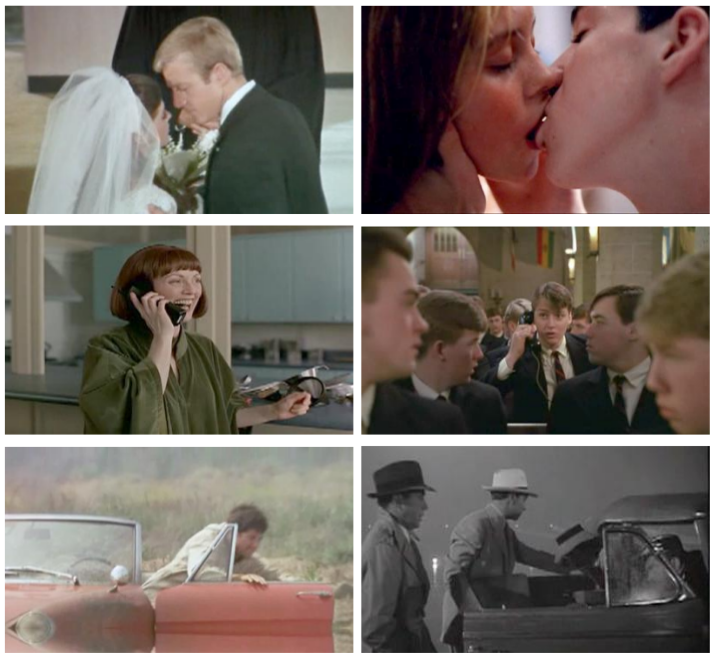
\includegraphics[width=1.0\linewidth]{fig1.png}
\end{center}
   \caption{
		   三类人类行为的现实样本:接吻,接电话,走出汽车。所有样本都通过从剧本对齐的电影中自动采集得到。
   }
\end{figure}

视频行为识别和静态图片行为识别面临着同样的困难。都需要处理明显的类内差异,背景混杂和遮挡问题。在静态图片
对象识别中,这些问题能够通过特征包(bag-of-features)描述方法\cite{17}和例如SVM这样的具有代表性的机器学习技术组合起
来得到相当好的处理。但是,这些结果是否能推广到现实中的人类行为识别中尚有待解答,例如,对故事片或者个人录像
进行识别。

基于近来图像分类的经验,我们在时空域上采用时空特征和广义的空域金字塔。
这使得我们可以用弱几何信息扩展时空特征包描述算法,并应用基于
运算核的学习技术(第3节)。我们在标准的基准\cite{15}上进行验证,发现这样
优于其它具有代表性的技术。然后我们转向现实视频中的行为分类问题,并展示
了我们采用的方法在电影中8类非常具有挑战性的行为类别上的可观结果。最后,
我们提出并评估一种行为学习和分类的全自动化配置,获取自动化标注的数据集合。

\subsection{相关工作}
我们的基于剧本的人类行为标注技术在本质上和一些近来采用文本信息从网络上
\cite{10,14}进行自动图像采集以及给图像中\cite{1}和视频中\cite{4}
的角色自动命名的文章相似。不同的是这项工作采用更加精细的文本分类工具来
克服文本中的行为差异。类似的,一些近期的方法探索采用特征包描述法
来进行行为识别\cite{3,6,13,15,19},但只是针对于控制下的简化场景设定。电影
中的行为的识别和定位近期在\cite{8}中在有限的数据集上得到处理,即人工标注
的两类行为。这里我们提出一种适用于数十个甚至更多的视觉行为类的自动标注。
我们的视频分类方法借鉴了一些图像识别方法\cite{2,9,12,20},并将空域金字塔
\cite{9}扩展到时空域金字塔。

\section{人类行为自动化标注}
这一节描述从电影中采集带标注人类行为的视频数据的自动过程。电影里有非常多样的
和大量的现实人类行为。然而,诸如接吻,接电话以及走出汽车等常见的行为类(图1)在一部
电影中只出现很少的次数。为了获取充足数量的行为样本以用于视觉训练,对上百个小时
的视频进行标注是必要的,人工标注是非常困难的一项任务。

为了避免人工标注的困难,我们采用\textit{电影剧本}(或简称``剧本'')。上百部著名的
电影\footnote{我们从\url{www.dailyscript.com},
\url{www.movie-page.com}以及\url{www.weeklyscript.com}上得到了上百个电影剧本。}的剧本是公开的并且在场景,
角色,转录对白和人类行为等方面提供了电影内容的描述。将剧本作为视频标注的方式已被
Everingham等人\cite{4}用于视频中的角色的自动命名。这里我们扩展这种思想,并应用基于
文本的剧本搜索来自动地收集人类行为的视频样本。

然而,从剧本中自动标注人类行为同样面临许多问题。首先,剧本通常没有时间信息,所以
必须要和视频进行对齐。其次,剧本中描述的行为并不是常常都和电影中的行为相关。最后,
行为恢复必须要处理文本中行为的大量实质性的变化。在这一节中我们在2.1节和2.2节中
处理这些问题,并在2.3节中采用提出的方法采集标注了人类行为的视频样本。得到的结果
作为第4节中训练和评估视觉行为分类器的数据集。

\subsection{剧本和视频行为的对齐}
电影剧本通常是普通文本格式并具有相似的结构。我们利用行缩进作为简单特征来将剧本
解析为独白,角色名称和场景描述(图2)。为了将剧本和视频对齐我们采用\cite{4}的方法
并利用另外从互联网上下载的电影字幕中的时间信息。如同\cite{4}一样,我们首先采用
单词匹配和动态编程对齐剧本和字幕中的对话段。然后将字幕中的时间信息转移到剧本中,
并推测场景描述之间的时间间隔,如图2所示。本文用于行为训练和分类的视频剪辑采用
场景描述之间的时间间隔来定义,可能包含多个行为或是没有行为的片段。为了指出一个
由剧本和字幕的不匹配造成的可能的不对齐的情况,我们将每一个场景描述和分数$a$关联
起来。$a$通过匹配字数与邻接对白的比例计算:$a=(\#matched words)/(\#all words)$。
(译者注:`\#' means ``number of''。)

时域不对齐可能由剧本和字幕不符造成。然而,由于可能的剧本和电影的不符,完美的字幕
对齐($a = 1$)并不能保证对视频行为的正确标注。

\begin{figure}[t]
\begin{center}
   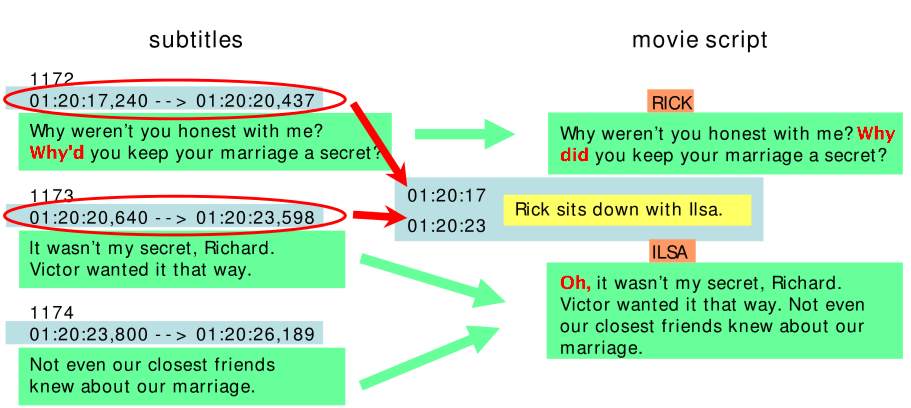
\includegraphics[width=1.0\linewidth]{fig2.png}
\end{center}
   \caption{
		   字幕和剧本中对话片段(绿色)的匹配示例。相邻对话片段的时间信息(蓝色)用来估计场景描述(黄色)的时间间隔。
   }
\end{figure}
\begin{figure}[h]
\begin{center}
   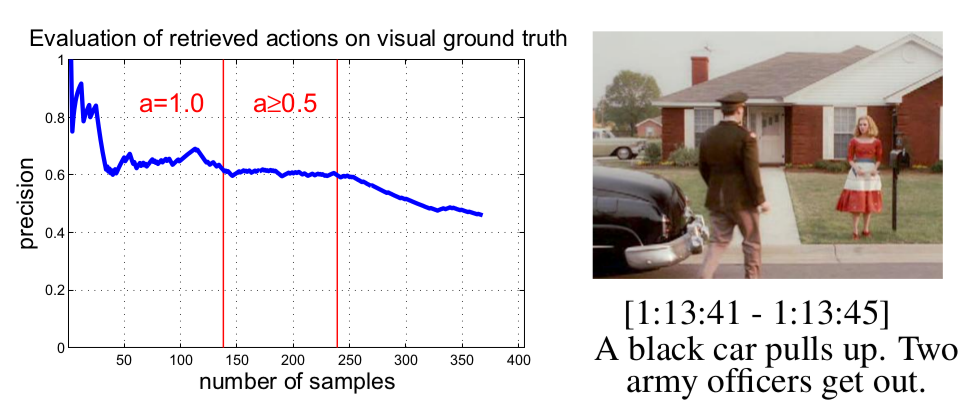
\includegraphics[width=1.0\linewidth]{fig3.png}
\end{center}
   \caption{
		   基于剧本的行为标注的评估。左:基于真实信息的行为标注精确度。右:``走出汽车‘’这一行为的视觉阳性误判的示例。
   }
\end{figure}

为了处理这个问题,我们人工地标注12部电影剧本中的上百个行为并在视觉真实情况上验证。147个具有正确文本对齐($a = 1$)的行为
中只有$70\%$和视频匹配。不匹配的样本可能是时间不对齐($10\%$),在视野之外($10\%$)或是完全不在视频中($10\%$)。字幕不对齐
($a < 1$)进一步降低了视觉精确度,如图3左所示。图3右展示了由于不在摄像头视野中所造成的``走出汽车''这一行为的一种典型
的``视觉阳性误判''。

\subsection{基于文本的人类行为恢复}
文本中的人类行为表达方式可能会有一些类内的差异。下面的例子描述了``走出汽车''这一行为的表达方式的一些类内差异:
``Will gets out of the Chevrolet.'',``A black car pulls up.Two army officers get out.'',``Erin exits her new truck.''。
而且,阳性误判不容易从阳性样本中分离出来,如``坐下''这一行为:``About to sit down,he freezes.'',``Smiling,he turns to 
sit down.But the smile dies on his face when he finds his place occupied by Ellie.''。因此,基于文本的行为恢复并不是
想象那么简单,通过像\cite{14}那样为了恢复图像中的对象而采用简单的关键字搜索是很难解决问题的。

为了处理人类行为文本描述方式的类内变化,我们采用基于机器学习的文本分类方法\cite{16}。分类器对剧本中的每个场景描述进行标记-
包含目标行为或没有包含目标行为。实现方法依赖于特征包模型,每个场景描述用一个高维特征空间中的稀疏向量表示。至于
特征我们采用一个N个单词的小窗口(N在2到8之间)中的单词,邻接单词对,以及非邻接单词对。少于3个训练文档支持的向量被删除掉。
分类方面我们采用一个和支持向量机等价的正则感知器\cite{21}。分类器在人工标注的场景描述集合上训练,参数(正则常数,窗口尺寸N,以及
判决门限)使用验证集合进行调整。

\begin{figure}[h]
\begin{center}
   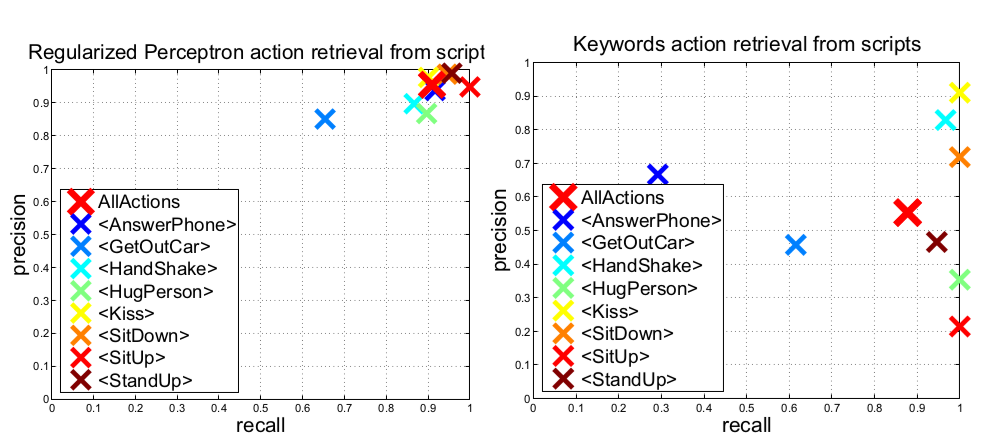
\includegraphics[width=1.0\linewidth]{fig4.png}
\end{center}
   \caption{
		   采用正则感知分类器(左)和正则表达式匹配(右)进行8类人类行为类恢复的结果对比。
   }
\end{figure}

我们在本文一直采用的8类电影中的行为上对基于文本的行为恢复进行评估:接电话,走出汽车,握手,拥抱,接吻,坐下去,坐起来,立正。
文本测试集合包含12个人工标准的电影剧本里的397个行为样本以及超过17000个非行为样本。文本训练集合从不同于测试集合的大量的剧本里
采样。我们比较正则感知分类器和通过匹配文本中的人类行为人工调整的正则表达式得到的结果。图4中的结果明显展示了文本分类器的优势。
平均precision-recall值分别是文本分类器[prec. 0.95/rec. 0.91]和正则表达式匹配[prec. 0.55/rec. 0.88]。

\subsection{人类行为视频数据集}
我们构建了两个视频训练集合(一个人工标注,一个自动标注),以及一个视频测试集合。这些视频包含了8类电影中行为(图10第一行)的视频
剪辑。在每种情况中我们首先使用自动剧本对齐技术(2.1节)。对于人工数据集和测试集合我们人工地从人工文本标注行为的剧本中选择了视觉
上正确的样本。自动化数据集包含了用2.2节描述的文本分类器自动恢复出来的样本。我们限定自动化训练集合为包含$a > 0.5$的行为,并将
视频长度限定在1000帧以内。人工和自动化的训练集合包含了12部电影\footnote{``American Beauty'',``Being John Malkovich'',``Big Fish'',
``Casablanca'',``The Crying Game'',``Double Indemnity'',``Forrest Gump'',``The Godfather'',``I Am Sam'',``Independence Day'',
``Pulp Fiction'' and ``Raising Arizona''}中的视频序列,测试集合来自另外20部电影\footnote{``As Good As It Gets'',``Big Lebowski'',
``Bringing Out The Dead'',``The Butterfly Effect'',``Dead Poets Society'',``Erin Brockovich'',``Fargo'',``Gandhi'',
 ``The Graduate'',``Indiana Jones And The Last Crusade'',``Its A Wonderful Life'',``Kids'',``LA Confidential'',``The Lord of The Ri
 ngs:Fellowship of the Ring'',``Lost Highway'',``The Lost Weekend'',``Mission To Mars'',``Naked City'',``The Pianist'' and 
 ``Reservoir Dogs''.}。我们的数据集(视频剪辑及相应的标注)可从\url{http://www.irisa.fr/vista/actions}下载。

\begin{figure}[h]
   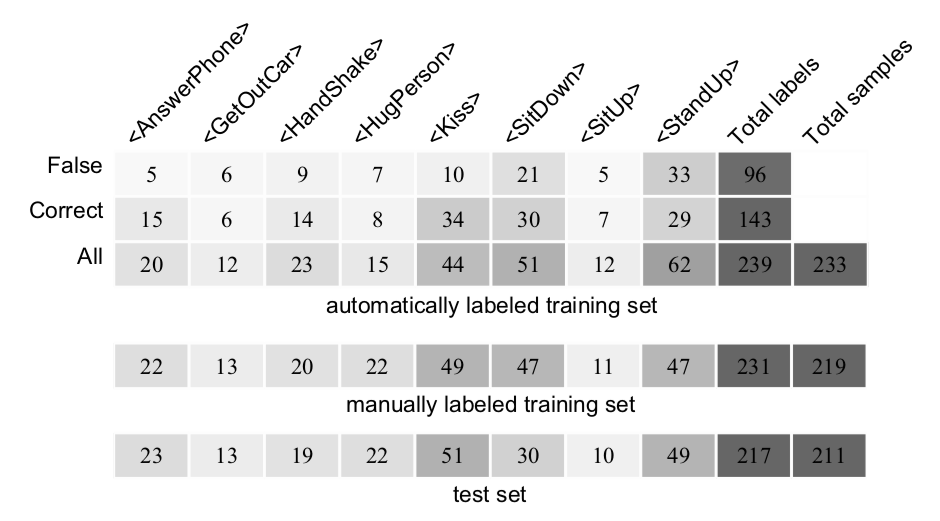
\includegraphics[width=1.0\linewidth]{table1.png}

  Table~1.~自动训练集合(上),人工训练集合(中)以及测试集合(下)中的行为标签数量。
\end{figure}

采用两个训练数据集的目的是对在监督学习设定和自动生成训练样本设定下的设别进行评估。注意到自动化训练集合中的样本和视频都没用
采用任何人工标注。不同子集的行为标签和行为类的分布在表1中给出。我们观察到正确标注视频的数量在自动化集合中占$60\%$。大多数错
误标注来自于剧本和视频不对齐以及少部分来自于文本分类器的附加错误。分类导致的错误训练标注的问题将在4.3节中进行讨论。

\section{行为识别中的视频分类}
这一节描述我们采用的行为分类方法。方法基于已存在的用于视频描述的特征包方法\cite{3,13,15}并将静态图片分类中
的优势扩展到视频中\cite{2,9,12}。Lazabnik等人\cite{9}发现空域金字塔,即空域场景布局的粗描述法,能够提升识别性能。基于
这种方法的一些成功的扩展包括单层金字塔的权重最优化\cite{2}以及广义空域网格\cite{12}的采用。这里我们基于这些想法提出
构建空域-时域网格的方法。方法的具体细节在下文描述。
\subsection{空域-时域特征}
稀疏空域-时域特征近来表现出在行为识别方面的良好性能\cite{3,6,13,15}。这些方法提供了一种紧凑的视频描述并且对背景混杂
,遮挡和尺寸变化具有耐受性。这里我们采用\cite{7},使用Harris操作的空域-时域扩展检测兴趣点。然而,和\cite{7}中采用
缩放选择不同,我们使用多尺度方法并在多层空域-时域尺寸$(\sigma^2_i,\tau^2_j)$上进行特征提取,
$\sigma_i=2^{(1+i)/2},i=1,...,6;\tau_j=2^{j/2},j=1,2$。这种选择受启发于减少计算复杂度,独立于尺寸选择人工痕迹以及近期
证明的采用密集尺寸缩放采样的良好识别性能。我们同时消除由于人工痕迹造成的位于判决边界的检测\cite{11}。图5展示了两帧人类
行为图像中检测出的兴趣点。
\begin{figure}[h]
\begin{center}
   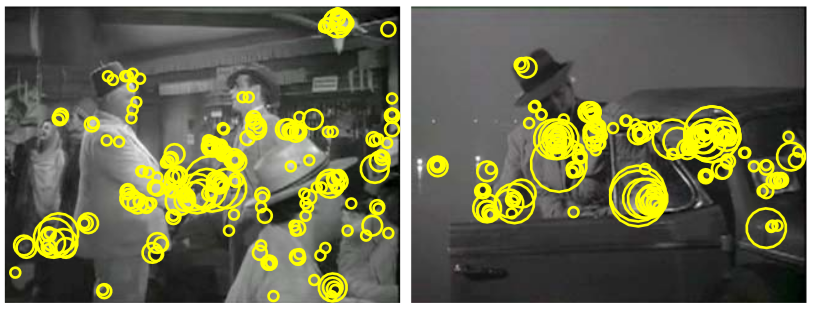
\includegraphics[width=1.0\linewidth]{fig5.png}
\end{center}
   \caption{
		   两帧带有人类行为:握手(左),走出汽车(右)中检测出的空域-时域兴趣点
   }
\end{figure}

为了使局部特征的动作和外貌特征化,我们计算邻接检测点空域-时域卷的直方图描述符。每一卷的大小$(\delta_x,\delta_y,\delta_z)$
和检测尺寸相关,$\delta_x,\delta_y=2k\sigma,\delta_t=2k\tau$。每一卷被分为一个$(n_x,n_y,n_t)$的立方体网格;对每一个立方体我们
分别计算粗梯度方向直方图(HoG)和光流直方图(HoF)。标准化后的直方图通过多列索引串联为HoG和HoF描述符矢量,这本质上和著名的SIFT描述符
相似。参数方面我们选择$k=9,n_x,n_y=3,n_t=2$。
\subsection{空域-时域特征包}
给定一个空域-时域特征集合,我们构建一个空域-时域特征包(BoF)。这需要构建一个视觉单词。在我们的实验中我们对一个从训练视频
中提取的100,000个特征子集采用k-means算法进行聚类。聚类数量设定为$k=4000$,经验显示这个参数能够给出良好结果,这和静态图像分类是一致
的。然后BoF表达式将每一个特征分配给最近的(欧式距离)单词,并在空域-时域卷上计算视觉单词出现次数直方图,空域-时域卷与整个视频序列
和空域-时域网格定义的子序列相关。如果有多个子集,不同的直方图串联成一个特征矢量,然后进行标准化。

空域维度方面我们采用一个$1\times1$网格-与标准BoF表达式相关,以及一个$2\times2$网格-在\cite{9}中展示出了优异的结果,一个水平
$h3\times1$网格\cite{12}以及一个垂直$v1\times3$网格。同时,我们实现一个密集$3\times3$网格以及一个中心聚焦$o2\times2$网格,邻接
单元$50\%$重叠。时域维度方面,我们将视频序列分为1到3非重叠时域箱,即$t_1$,$t_2$及$t_3$分箱。$t_1$表示标准BoF方法。我们也实现了
一个中心聚焦的$ot_2$分箱。注意到重叠部分的网格位于中心的特征权重更大。

6个空域网格和4个时域分箱的组合形成24种可能的空域-时域网格。图6描述了一些被证明是对行为识别有用的网格。每一个空域-时域网格的组合
使用一个HoG或HoF描述符,封装进下面介绍的一个通道中。

\begin{figure}[h]
\begin{center}
   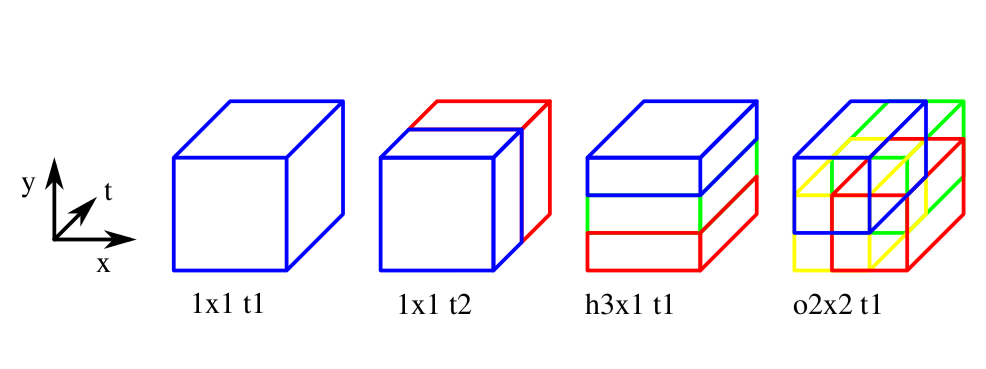
\includegraphics[width=1.0\linewidth]{fig6.png}
\end{center}
   \caption{
		   一些空域-时域网格的示例。
   }
\end{figure}

\subsection{Non-linear Support Vector Machines}
为了进行分类,我们采用非线性支持向量机和一个鲁棒地联合通道的多通道$\chi^2$核\cite{20}。采用多通道高斯核:
\[K(H_i,H_j)=exp(-\sum_{c\in{C}}\frac{1}{A_c}D_c(H_i,H_j))\]
$H_i={h_{in}};H_j={h_{jn}}$是通道$c$的直方图,$D_c(H_i,H_j)$是$\chi^2$距离:
\[D_c(H_i,H_j)=\frac{1}{2}\sum^V_{n=1}\frac{(h_{in}-h_{jn})^2}{h_{in}+h_{jn}}\]
V是单词大小。参数$A_c$是一个通道的所有的训练样本之间的距离的平均值\cite{20}。针对给定的训练集合的$C$通道的最佳集合
通过贪心算法找到。从空通道集合开始所有的可能的附加核删除通道都被评估,直到达到最大值。在多类分类方面我们使用one-against-all方法。
\section{Experimental results}
\subsection{Evaluation of spatio-temporal grids}
\subsection{Comparison to the state-of-the-art}
\subsection{Robustness to noise in the training data}
\subsection{Action recognition in real-world videos}
\section{Conclusion}
{\small
\bibliographystyle{ieee}
\bibliography{bib}
}

\end{document}
